\documentclass[../../main/main.tex]{subfiles}
\graphicspath{{./figures/}}

\dominitoc
\faketableofcontents

% \renewcommand{\mtcSfont}{\small\bfseries}
% \renewcommand{\mtcSSfont}{\footnotesize}
\mtcsettitle{minitoc}{}
\mtcsetrules{*}{off}

\makeatletter
\renewcommand{\@chapapp}{\'Electrocin\'etique -- chapitre}
\renewcommand{\chaplett}{E}
\renewcommand{\thefigure}{\chaplett\arabic{figure}}
\makeatother

% \toggletrue{student}
% \toggletrue{corrige}
% \renewcommand{\mycol}{black}
% \renewcommand{\mycol}{gray}

\hfuzz=5.003pt

\begin{document}
\setcounter{chapter}{5}

\settype{book}
\settype{prof}
\settype{stud}

\chapter{Circuits électriques en régime sinusoïdal forcé}

\vspace*{\fill}

\begin{tcn}(appl)<ctc>"somm"'t'{Sommaire}
	\let\item\olditem
	\vspace{-15pt}
	\minitoc
	\vspace{-25pt}
\end{tcn}

\begin{tcn}[sidebyside](appl)<ctb>"how"'t'{Capacités exigibles}
	\begin{itemize}[label=\rcheck]
		\item Établir et connaître l'impédance d'une résistance, d'un
		      condensateur, d'une bobine.
		\item Oscillateur électrique ou mécanique soumis à une excitation
		      sinusoïdale.
	\end{itemize}
	\tcblower
	\begin{itemize}[label=\rcheck]
		\item Remplacer une association série ou parallèle de deux impédances par
		      une impédance équivalente.
		\item Utiliser la représentation complexe pour étudier le régime forcé.
	\end{itemize}
\end{tcn}

\vspace*{\fill}
\newpage
\vspace*{\fill}

%\vspace{-15pt}
\begin{tcn}[%
		sidebyside, fontupper=\small, fontlower=\small
	](appl)<ctb>"chek"'t'{L'essentiel}
	\begin{tcn}[nsp](defi)<ctc>'t'{Définitions}
		\vspace{-25pt}
		\tcblistof[\subsubsection*]{defi}{\hspace*{4.8pt}}
	\end{tcn}
	\begin{tcn}[nsp](rapp)<ctc>'t'{Rappels}
		\vspace{-25pt}
		\tcblistof[\subsubsection*]{rapp}{\hspace*{4.8pt}}
	\end{tcn}
	\begin{tcn}[nsp](prop)<ctc>'t'{Propriétés}
		\vspace{-25pt}
		\tcblistof[\subsubsection*]{prop}{\hspace*{4.8pt}}
		% \tcblistof[\subsubsection*]{loi}{\hspace*{4.8pt}}
		% \tcblistof[\subsubsection*]{theo}{\hspace*{4.8pt}}
	\end{tcn}
	% \begin{tcn}[nsp](loi)<ctc>'t'{Lois}
	% 	\tcblistof[\subsubsection*]{loi}{\hspace*{4.8pt}}
	% \end{tcn}
	% \begin{tcn}[nsp](coro)<ctc>'t'{Corollaires}
	%   \tcblistof[\subsubsection*]{coro}{\hspace*{4.8pt}}
	% \end{tcn}
	% \begin{tcn}[nsp](demo)<ctc>'t'{Démonstrations}
	% 	\tcblistof[\subsubsection*]{demo}{\hspace*{4.8pt}}
	% 	\tcblistof[\subsubsection*]{prev}{\hspace*{4.8pt}}
	% \end{tcn}
	% \begin{tcn}[nsp](inte)<ctc>'t'{Interprétations}
	% 	\tcblistof[\subsubsection*]{inte}{\hspace*{4.8pt}}
	% \end{tcn}
	% \begin{tcn}[nsp](impl)<ctc>'t'{Implications}
	% 	\vspace{-25pt}
	% 	\tcblistof[\subsubsection*]{impl}{\hspace*{4.8pt}}
	% \end{tcn}
	% \begin{tcn}[nsp](tool)<ctc>'t'{Outils}
	% 	\tcblistof[\subsubsection*]{tool}{\hspace*{4.8pt}}
	% \end{tcn}
	% \begin{tcn}[nsp](nota)<ctc>'t'{Notations}
	% 	\tcblistof[\subsubsection*]{nota}{\hspace*{4.8pt}}
	% \end{tcn}
	% \begin{tcn}[nsp](appl)<ctc>'t'{Applications}
	% 	\tcblistof[\subsubsection*]{appl}{\hspace*{4.8pt}}
	% \end{tcn}
	% \begin{tcn}[nsp](rema)<ctc>'t'{Remarques}
	%   \tcblistof[\subsubsection*]{rema}{\hspace*{4.8pt}}
	% \end{tcn}
	% \begin{tcn}[nsp](exem)<ctc>'t'{Exemples}
	%   \tcblistof[\subsubsection*]{exem}{\hspace*{4.8pt}}
	% \end{tcn}
	% \begin{tcn}[nsp](ror)<ctc>"hart"'t'{Points importants}
	%   \tcblistof[\subsubsection*]{ror}{\hspace*{4.8pt}}
	% \end{tcn}
	% \begin{tcn}[nsp](impo)<ctc>'t'{Erreurs communes}
	%   \tcblistof[\subsubsection*]{impo}{\hspace*{4.8pt}}
	% \end{tcn}
	\tcblower
	% \begin{tcn}[nsp](defi)<ctc>'t'{Définitions}
	%   \tcblistof[\subsubsection*]{defi}{\hspace*{4.8pt}}
	% \end{tcn}
	% \begin{tcn}[nsp](rapp)<ctc>'t'{Rappels}
	%   \tcblistof[\subsubsection*]{rapp}{\hspace*{4.8pt}}
	% \end{tcn}
	% \begin{tcn}[nsp](prop)<ctc>'t'{Propriétés}
	% \tcblistof[\subsubsection*]{prop}{\hspace*{4.8pt}}
	% \tcblistof[\subsubsection*]{loi}{\hspace*{4.8pt}}
	% \tcblistof[\subsubsection*]{theo}{\hspace*{4.8pt}}
	% \end{tcn}
	% \begin{tcn}[nsp](coro)<ctc>'t'{Corollaires}
	%   \tcblistof[\subsubsection*]{coro}{\hspace*{4.8pt}}
	% \end{tcn}
	\begin{tcn}[nsp](demo)<ctc>'t'{Démonstrations}
		\vspace{-25pt}
		\tcblistof[\subsubsection*]{demo}{\hspace*{4.8pt}}
		% \tcblistof[\subsubsection*]{prev}{\hspace*{4.8pt}}
	\end{tcn}
	% \begin{tcn}[nsp](inte)<ctc>'t'{Interprétations}
	% 	\tcblistof[\subsubsection*]{inte}{\hspace*{4.8pt}}
	% \end{tcn}
	% \begin{tcn}[nsp](impl)<ctc>'t'{Implications}
	% 	\tcblistof[\subsubsection*]{impl}{\hspace*{4.8pt}}
	% \end{tcn}
	\begin{tcn}[nsp](tool)<ctc>'t'{Outils}
		\vspace{-25pt}
		\tcblistof[\subsubsection*]{tool}{\hspace*{4.8pt}}
	\end{tcn}
	% \begin{tcn}[nsp](nota)<ctc>'t'{Notations}
	% 	\tcblistof[\subsubsection*]{nota}{\hspace*{4.8pt}}
	% \end{tcn}
	% \begin{tcn}[nsp](odgr)<ctc>'t'{Ordres de grandeur}
	% 	\tcblistof[\subsubsection*]{odgr}{\hspace*{4.8pt}}
	% \end{tcn}
	\begin{tcn}[nsp](appl)<ctc>'t'{Applications}
		\vspace{-25pt}
		\tcblistof[\subsubsection*]{appl}{\hspace*{4.8pt}}
	\end{tcn}
	% \begin{tcn}[nsp](rema)<ctc>'t'{Remarques}
	%   \tcblistof[\subsubsection*]{rema}{\hspace*{4.8pt}}
	% \end{tcn}
	% \begin{tcn}[nsp](exem)<ctc>'t'{Exemples}
	% 	\tcblistof[\subsubsection*]{exem}{\hspace*{4.8pt}}
	% \end{tcn}
	\begin{tcn}[nsp](ror)<ctc>"hart"'t'{Points importants}
		\vspace{-25pt}
		\tcblistof[\subsubsection*]{ror}{\hspace*{4.8pt}}
	\end{tcn}
	\begin{tcn}[nsp](impo)<ctc>'t'{Erreurs communes}
		\vspace{-25pt}
		\tcblistof[\subsubsection*]{impo}{\hspace*{4.8pt}}
	\end{tcn}
\end{tcn}

\vspace*{\fill}

\newpage

\section{Présentation du régime forcé}
\subsection{Définition}

Jusque-là en électrocinétique, nous avons étudié la réponse d'un circuit
(c'est-à-dire la tension de sortie) de systèmes linéaires soit libres, soit à un
forçage constant. On s'intéresse maintenant à la physique de ces systèmes
lorsqu'ils sont soumis à des forçages sinusoïdaux.

\begin{tcb}(defi){Régimes de forçages}
	\begin{itemize}
		\item \leftcenters{%
		      \textbf{Libre}~:
		      }{%
		      $\DS \sum_{i} f_i(t) \dv[i]{y}{t} =
			      \psw{\underbracket[1pt]{0}_{\mathclap{\text{libre}}}}
		      $
		      }%
		      \vspace{-15pt}
		\item \leftcenters{%
		      \textbf{Forçage constant}~:
		      }{%
		      $\DS \sum_{i} f_i(t) \dv[i]{y}{t} =
			      \psw{\underbracket[1pt]{K}_{\mathclap{\text{forçage cst.}}}}
		      $
		      }%
		      \vspace{-15pt}
		\item \leftcenters{%
		      \textbf{Forçage sinusoïdal}~:
		      }{%
		      $\DS \sum_{i} f_i(t) \dv[i]{y}{t} =
			      F(t) =
			      \psw{\underbracket[1pt]{F_0 \cos(\wt + \f_0)}_{\mathclap{\text{forçage sinusoïdal}}}}
		      $
		      }%
	\end{itemize}
\end{tcb}

\begin{tcb}(rapp){Réponses système amorti}
	\begin{itemize}
		\item
		      \leftcenters{%
			      \textbf{Libre}~: % on avait
		      }{%
			      \psw{$y\ind{libre}(t) = y_h(t) \opto{}{t\to\infty} 0$}
		      }%
		\item
		      \leftcenters{%
			      \textbf{Forçage constant}~: % on avait
		      }{%
			      \psw{$y\ind{forcé}(t) = y_h(t) + y_p \opto{}{t\to\infty} y_p$}
		      }%
		      \smallbreak
		      avec $y_p = \cte$, \xul{de la même forme que le forçage}.
	\end{itemize}
\end{tcb}

\subsection{Réponse d'un système en RSF}
\begin{tcb*}(prop){Système amorti en RSF}
	\begin{itemize}
		\item \leftcenters{%
			      \textbf{Forçage sinusoïdal}~: % on obtient
		      }{%
			      \psw{$y\ind{forcé}(t) = y_h(t) + y_p(t) \opto{}{t\to\infty} y_p(t)$}
		      }%
		      \smallbreak
		      Avec $y_p(t)$ \textbf{de la même forme que le forçage}~: on cherchera
		      \psw{%
			      \[
				      \boxed{y_p(t) = Y_0 \cos(\wt + \f)}
			      \]
		      }%
		      \begin{center}
			      \sswitch{%
				      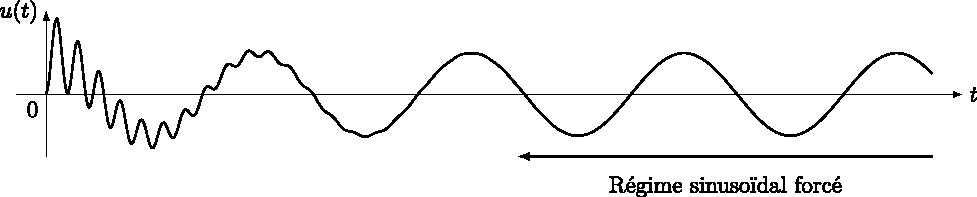
\includegraphics[width=.7\linewidth, draft=true]{rsf_transi}
			      }{%
				      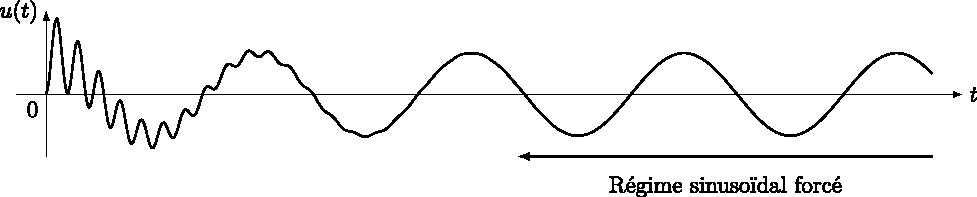
\includegraphics[width=.7\linewidth]{rsf_transi}
			      }%
			      \captionof{figure}{Exemple d'un signal en RSF.}
		      \end{center}
	\end{itemize}
\end{tcb*}

\begin{tcb}(defi){Régime sinusoïdal forcé}
	Ainsi, concrètement on appelle \textbf{régime sinusoïdal forcé} le
	\textbf{régime permanent} d'un système amorti soumis à une \textbf{entrée
		sinusoïdale}.
\end{tcb}

\begin{tcb}(rema)<lftt>{Régimes permanents}
	\begin{itemize}
		\item On est en \textbf{régime transitoire} tant que $y_h(t)$ n'est
		      \textbf{pas négligeable} devant $y_p(t)$. Une fois l'\textbf{amortissement
			      terminé}, quand $y\ind{forcé}(t) = y_p(t)$, on est en \textbf{régime
			      permanent}.
		\item Précédemment, on avait un forçage constant, soit $\w = 0 \Lra f = 0
			      \Ra F (\bcancel{t})$~; c'est ce qu'on appelle le \textbf{régime permanent
			      \xul{continu}}.
		\item Dorénavant, on étudie un \textbf{régime permanent \xul{variable}}.
	\end{itemize}
\end{tcb}

\begin{tcb}[label=prop:sortiersf](ror){Signaux de sorties en RSF}
	Pour un signal d'entrée
	\psw{%
		\[
			e(t) = E_0 \cos(\wt)
			\quad(\text{ou}\quad
			\eta(t) = \eta_0\cos(\wt))
		\]
	}%
	les différentes tensions et intensités dans le circuit oscilleront \textbf{à
		la même pulsation $\w$}~:
	\psw{%
		\[
			u(t) = U\cos(\wt+\f_u)
			\qet
			i(t) = I\cos(\wt+\f_i)
		\]
	}%
	où $U$, $I$ et $\f_{u,i}$ sont des grandeurs dépendant du système et de
	la pulsation $\w$.
	\begin{center}
		\bfseries
		L'objectif de ce chapitre est de donc de savoir déterminer $U$ et $\f$.
	\end{center}
\end{tcb}

\begin{tcb}[label=ror:CIounon](impo){Grandeurs à déterminer}
	Dans le cas du \textbf{régime libre}, une solution $y_h(t)$ fait intervenir une ou
	plusieurs \textbf{constantes d'intégration}, que l'on détermine avec les
	\textbf{conditions initiales}.
	\bigbreak
	En revanche, comme précédemment, les \textbf{constantes de $y_p(t)$}, ici
	$Y_0$ et $\f$, dépendent des \textbf{paramètres du système}, pas des
	conditions initiales~! En électricité, ça sera $R$, $L$, $C$, $E_0$, $\w$…
	% \smallbreak \centering\large
	% dépendent du circuit (ici, $R$, $C$, $\w$ et $E_0$).
\end{tcb}

% Nous avons alors observé la présence d'un régime
% \textbf{transitoire} suivi d'un régime \textbf{permanent \xul{constant}}.
% Dans ce chapitre, nous allons voir la réponse d'un circuit à une entrée
% \textbf{sinusoïdale}, qui donnera lieu à un régime transitoire suivi d'un régime
% \textbf{permanent \xul{sinusoïdal}}. D'une manière générale, on se
% concentre sur la réponse du système une fois le régime permanent établi. On
% définit donc

% \begin{tcb}[label=def:rsf](defi){Régime sinusoïdal forcé}
% 	On appelle \textbf{régime sinusoïdal forcé} le \textbf{régime permanent} d'un
% 	circuit électrique soumis à une \textbf{entrée sinusoïdale}.
% 	\smallbreak
% 	Dans tout le chapitre, on supposera donc que l'entrée est allumée depuis une
% 	durée suffisamment longue pour considérer que le \textbf{régime transitoire
% 		est terminé}.
% 	\begin{center}
% 		\sswitch{%
% 			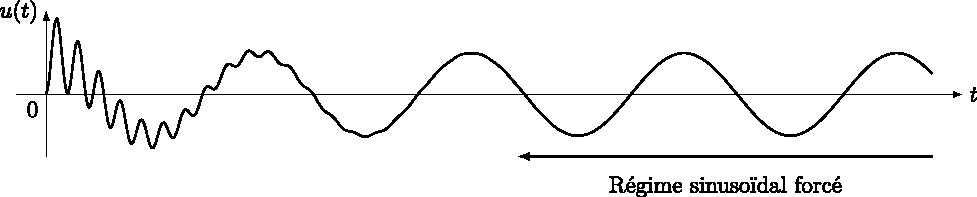
\includegraphics[width=.7\linewidth, draft=true]{rsf_transi}
% 		}{%
% 			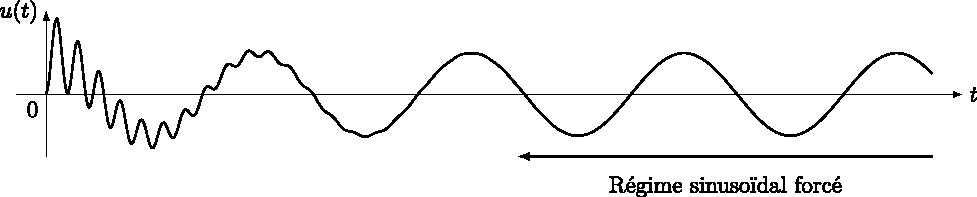
\includegraphics[width=.7\linewidth]{rsf_transi}
% 		}%
% 		\captionof{figure}{Exemple d'un signal en RSF.}
% 	\end{center}
% \end{tcb}

\vspace{-10pt}
\subsection{Notions de signaux périodiques}
\subsubsection{Période}
\begin{tcb}(defi){Période}
	\psw{%
		\[
			s(t) \quad \text{périodique}
			\equiv
			\exists T~: \forall t \in \Rb^{+}, s(t+T) = s(t)
		\]
	}%
	\vspace{-15pt}
\end{tcb}
\begin{tcb}(appl)<lftt>{Périodicité}
	Montrer que le signal $s(t) = A \sin(\wt)$ a une période $T =
		\frac{2\pi}{\w}$.
	\tcblower
	\psw{%
		\[
			s \left( t + \frac{2\pi}{\w} \right) =
			A \left( \w \left( t + \frac{2\pi}{\w} \right) \right) =
			A \sin(\wt + 2\pi) = A \sin(\wt)
			\qed
		\]
	}%
	\vspace{-15pt}
\end{tcb}

\subsubsection{Moyenne}
\begin{tcb}(defi){Valeur moyenne}
	Pour un \textbf{signal périodique} $s(t)$, on définit sa valeur moyenne
	$\moy{s(t)}$ par
	\psw{%
		\[
			\moy{s(t)} = \frac{1}{T}\int _{0}^{T} s(t) \dd{t}
		\]
	}%
	\vspace{-15pt}
\end{tcb}

\begin{tcb}[sidebyside, lefthand ratio=.4](appl)<lftt>{Moyenne d'un cosinus décalé}
	Calculer la valeur moyenne du signal
	\[
		s(t) = S_0 + A\cos(\wt)
	\]
	\begin{center}
		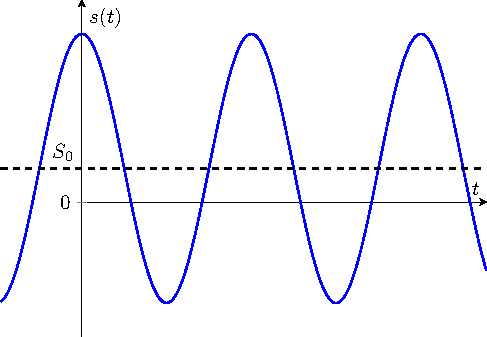
\includegraphics[width=\linewidth]{moy_cos-S0}
		\captionof{figure}{$s(t) = S_0 + A\cos(\wt)$}
	\end{center}
	\tcblower
	\psw{%
		\begin{align*}
			\moy{s(t)}         & =
			\frac{1}{T} \int_{0}^{T} (S_0 + A\cos(\wt))\dd{t}
			\\&=
			\frac{1}{T} \left( \int_{0}^{T} S_0 \dd{t} +
			\int_{0}^{T} A \cos(\wt)\dd{t} \right)
			\\&=
			\frac{1}{T} \left( [S_0t]_0^{T} +
			\left[ \frac{A}{\w} \sin(\wt) \right]_0^{T} \right)
			\\&=
			\frac{1}{T} \left( S_0(T-0) +
			\underbracket[1pt]{\frac{A}{\w} \left( \sin(\w T) - \sin(\w \times 0) \right)}_{=0} \right)
			\\&=
			\frac{1}{T} S_0T
			\\\Lra
			\Aboxed{\moy{s(t)} & = S_0}
			\qed
		\end{align*}
	}%
	\vspace{-15pt}
\end{tcb}

\begin{tcb}[cnt, bld](ror){Moyenne d'un signal sinusoïdal}
	Un signal purement sinusoïdal a une moyenne nulle.
\end{tcb}

\subsubsection{Valeur efficace}
Ainsi, si on envoie une tension sinusoïdale dans un circuit et qu'on mesure la
moyenne de la tension reçue, on trouvera une tension nulle. Pourtant, l'énergie
transmise n'est pas nulle~! C'est parce que les électrons réagissent à la fois
aux tensions positives et négatives du signal, et ce pourquoi on obtient $\Ec_C
	= \frac{1}{2}Cu_C{}^{2}$~: l'\textbf{énergie est proportionnelle au carré des
	signaux}.
\begin{tcb*}(defi){Valeur efficace}
	On définit la valeur efficace d'un signal \textbf{périodique} par
	\psw{%
		\[
			s \ind{eff} = \sqrt{\moy{s^{2}(t)}}
		\]
	}%
	Ainsi, $s \ind{eff}^{2}$ représente l'\textbf{énergie moyenne du signal}.
\end{tcb*}
% Notamment, la valeur de
% \SI{230}{V} pour la tension secteur est la valeur \textit{efficace}~: c'est une
% tension sinusoïdale qui oscille entre des valeurs de $\SI{\pm 325}{V}$.

\begin{tcb*}[sidebyside, lefthand ratio=.4](appl)<lftt>{Calcul de valeur efficace}
	Calculer la valeur efficace du signal
	\[
		s(t) = A \cos(\wt)
	\]
	\begin{center}
		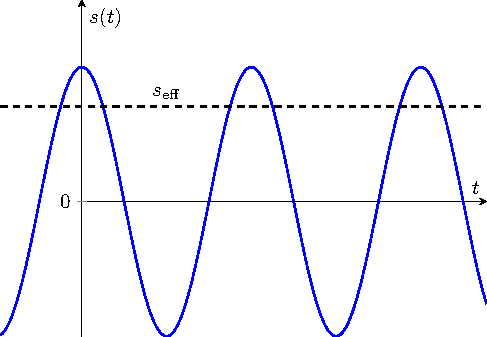
\includegraphics[width=\linewidth]{veff_cos}
		\captionof{figure}{$s \ind{eff}$ de $A\cos(\wt)$.}
	\end{center}
	\tcblower
	\psw{%
		\begin{align*}
			\moy{s^{2}(t)}      & =
			\frac{1}{T} \int_{0}^{T} \left( A^{2}\cos^{2}(\wt) \right) \dd{t}
			\\ &=
			\frac{A^{2}}{T} \left( \int_{0}^{T} \frac{1}{2} \dd{t} +
			\int_{0}^{T} \frac{\cos(2\wt)}{2} \dd{t}\right)
			\\ &=
			\frac{A^{2}}{T}
			\Bigg(
			\underbracket[1pt]{\left[ \frac{1}{2}t \right]_0^{T}}_{=\frac{T}{2}} +
			\underbracket[1pt]{\left[ \frac{1}{2} \frac{A}{2\w} \sin(2\wt) \right]_0^{T}}_{=0}
			\Bigg)
			\\[-18pt] &=
			\frac{A^{2}}{2}
			\\\Lra
			\Aboxed{s \ind{eff} & = \frac{A}{\sqrt{2}}}
			\qed
		\end{align*}
	}%
	\vspace{-15pt}
\end{tcb*}

% \begin{tcb*}(impo)<lftt>{Valeur efficace autres signaux}
% 	Il n'y a pas toujours de rapport $\sqrt{2}$ entre amplitude et valeur
% 	efficace~! Pour un signal triangle, la valeur efficace est $A/\sqrt{3}$, et
% 	pour un créneau pur sa valeur efficace est son amplitude $A$.
% \end{tcb*}

\subsection{Passage en complexes}
\begin{tcb*}[sidebyside, righthand ratio=.4](tool){Représentation complexe}

	\psw{%
		\begin{DispWithArrows*}[groups]
			y(t) &= Y_0 \cos(\wt+\f)
			\Arrow{Passage $\Cb$}
			\\\Lra
			\yu(t) &= Y_0 \exr^{\jj (\wt+\f)}
			\Arrow{Séparation de $t$}
			\\\Lra
			\yu(t) &= \underbracket[1pt]{Y_0\exr^{\jj \f}}_{=\cte}\cdot\exr^{\jwt}
			\Arrow{Réécriture}
			\\\Lra
			\Aboxed{\yu(t) &= \Yu\exr^{\jwt}}
			\\\text{avec} \quad
			\Aboxed{\Yu &= Y_0\exr^{\jj \f}}
			\Ra
			\left\{
			\begin{array}{ll}
				Y_0 & = \abs{\Yu}
				\\
				\f  & = \arg*{\Yu}
			\end{array}
			\right.
		\end{DispWithArrows*}
	}%
	Comme \textbf{on connaît $\w$} la pulsation du signal d'entrée, on ne
	\textbf{cherchera que l'amplitude complexe} $\Yu$, qu'on peut représenter
	dans le plan complexe~:
	\tcblower
	\begin{center}
		\sswitch{%
			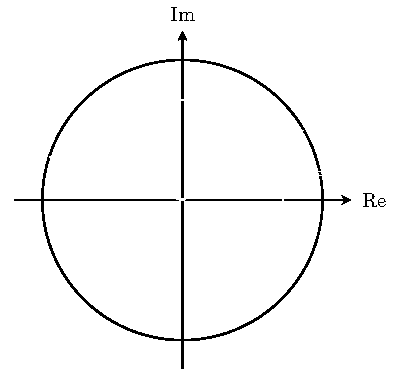
\includegraphics[width=\linewidth]{cplx_pres-xy_stud}
		}{%
			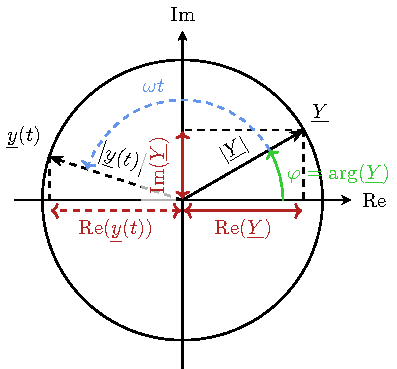
\includegraphics[width=\linewidth]{cplx_pres-xy_prof}
		}%
		\captionof{figure}{Représentation de $\Yu$.}
	\end{center}
\end{tcb*}

\begin{tcb}(impo)<lftt>{Passage en complexes}
	Le passage ne fonctionne \textbf{que si le signal est un cosinus}~! Dans le
	cas contraire, \textbf{on se ramène à un cosinus} par un terme de phase
	($\sin(x+\frac{\pi}{2}) = \cos(x)$).
	\smallbreak
	En effet, l'opération inverse du passage en complexe est la partie réelle~:
	\psw{%
		\begin{align*}
			y(t) & = \Re(\yu(t)) = \Re(Y_0\exr^{\jj (\wt + \f)})
			\\\Lra
			y(t) & = \Re(Y_0(
			\cos(\wt+\f) + \jj \sin(\wt+\f))) = Y_0\cos(\wt + \f)
		\end{align*}
	}%
	\vspace{-15pt}
	% Il faut donc bien que l'on ait transformé un cosinus et non un sinus~!
\end{tcb}

\begin{tcb*}[breakable](rapp){Outils mathématiques}
	Soit $\zu = x + \jj y$ un nombre complexe. On peut le représenter comme un
	\textbf{vecteur dans le plan complexe}. On retrouve alors facilement les
	résultats suivants~:
	\tcbsubtitle{\fatbox{\textbf{Module}}}
	Le module d'un nombre complexe est \textbf{la norme du vecteur dans le plan
		complexe}. On a
	\[
		\psw{%
			\boxed{\abs{\zu} = \sqrt{x^2 + y^2}}
		}%
		\qqet
		\forall (\xul{z_1}, \xul{z_2}) \in \Cb^2,
		\qquad
		\psw{%
			\abs{\frac{\xul{z_1}}{\xul{z_2}}} =
			\frac{\abs{\xul{z_1}}}{\abs{\xul{z_2}}}
		}%
	\]
	\tcbsubtitle{\fatbox{\textbf{Argument}}}
	Son argument est \textbf{l'angle dans le plan complexe}~:
	$\arg*{\zu} = \f$. On retrouve alors
	% c'est-à-dire ici $\arg*{\Yu} = \f$.
	\begin{gather*}
		\psw{%
			\cos(\arg*{\zu}) = \frac{\Re(\zu)}{\abs{\zu}}
			\qquad
			\sin(\arg*{\zu}) = \frac{\Im(\zu)}{\abs{\zu}}
			\qquad
			\tan(\arg*{\zu}) = \frac{\Im(\zu)}{\Re(\zu)}
		}%
		\\\beforetext{Mais encore,}
		\forall (\xul{z_1}, \xul{z_2}) \in \Cb^2,
		\qquad
		\psw{%
			\boxed{
				\arg*{ \frac{\xul{z_1}}{\xul{z_2}} } =
				\arg*{\xul{z_1}} - \arg*{\xul{z_2}}
			}%
		}%
		\vspace{-15pt}
	\end{gather*}
	\begin{isd}[interior hidden](rapp)
		\tcbsubtitle{\fatbox{\textbf{Dérivée}}}
		\vspace{-10pt}
		\[
			\psw{%
				\dv{\yu}{t} = \dv{\Yu\exr^{\jwt}}{t} = \jw \cdot \Yu\exr^{\jwt}
				\Lra
				\boxed{\dv{\yu}{t} = \jw \yu(t)}
			}
		\]
		\tcblower
		\tcbsubtitle{\fatbox{\textbf{Primitive}}}
		\vspace{-10pt}
		\[
			\psw{%
				\int \yu = \int \Yu\exr^{\jwt} = \frac{\Yu\exr^{\jwt}}{\jw}
				\Lra
				\boxed{\int \yu(t) = \frac{\yu(t)}{\jw}}
			}
		\]
	\end{isd}
\end{tcb*}

\begin{tcb*}[breakable](impo){Arguments en physique complexe}
	Par convention, on choisit d'exprimer \textbf{tous les angles dans}
	$[-\pi;\pi]$. Pour trouver la valeur d'un angle, on procède de la même manière
	que d'habitude~: avec de la trigonométrie. Notamment, en connaissant
	$\Re(\Yu)$ et $\Im(\Yu)$, on cherchera souvent à calculer
	$\tan(\arg*{\Yu})$, puis à \textbf{appliquer arctan} pour retrouver $\f =
		\arg*{\Yu}$.
	\bigbreak
	\textbf{Cependant}, arctan est définie telle que
	$\begin{array}{ccccc}
			\arctan & : & ]-\infty;\infty[ & \to &
			\left] -\frac{\pi}{2} ; \frac{\pi}{2} \right[ \\
		\end{array}$
	% $\arctan : ]-\infty;\infty[ \to \left]
	% -\frac{\pi}{2} ; \frac{\pi}{2} \right[$,
	c'est-à-dire que
	\[
	\psw{%
	\boxed{  \arctan(\tan(\th)) = \th \Lra \th \in
	\left]-\frac{\pi}{2} ; \frac{\pi}{2} \right[}
		}%
		\]
		\vspace{-15pt}
		\begin{center}
			\begin{tabularx}{\linewidth}{YY}
				\sswitch{%
					{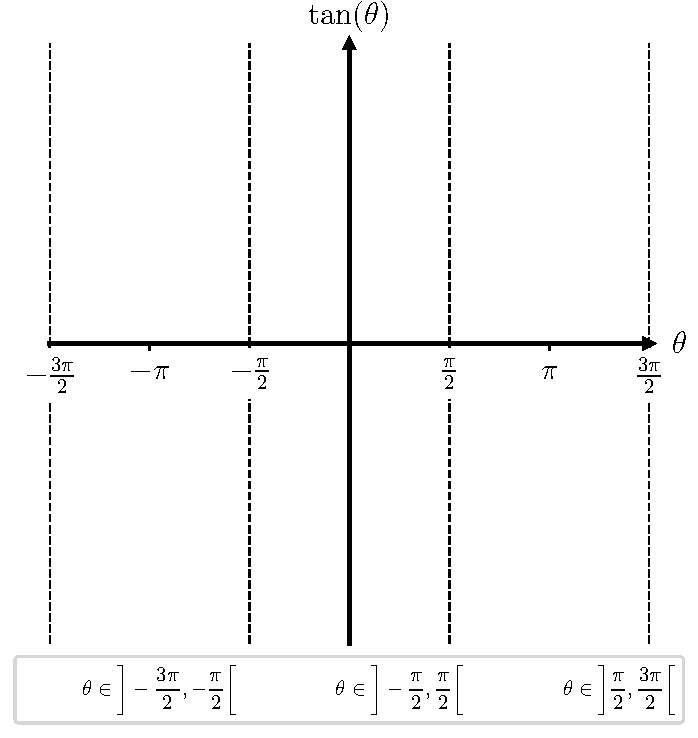
\includegraphics[width=0.85\linewidth]{fig_tan_stud}}
				}{%
					{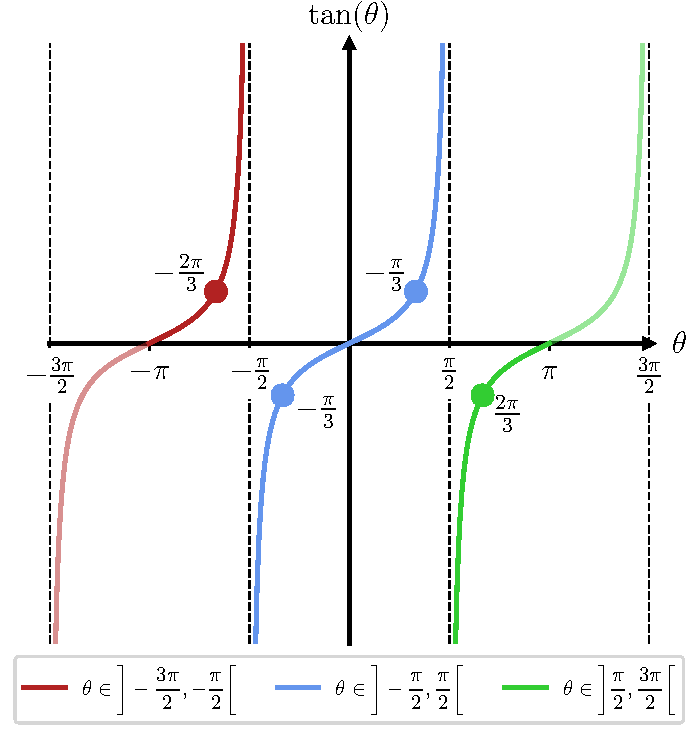
\includegraphics[width=0.85\linewidth]{fig_tan_prof}}
				}%
				\captionof{figure}{$\tan(\th)$}
				 &
				\sswitch{%
					{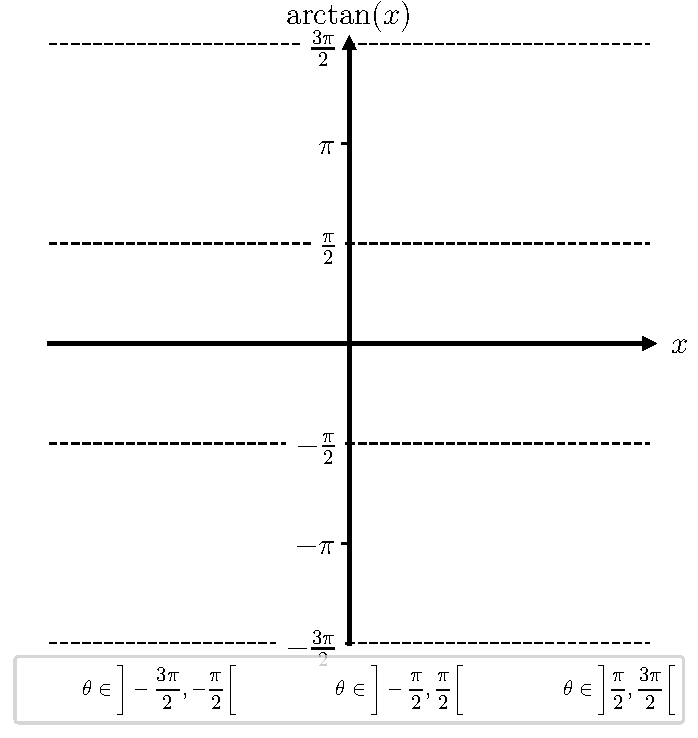
\includegraphics[width=0.85\linewidth]{fig_atan_stud}}
				}{%
					{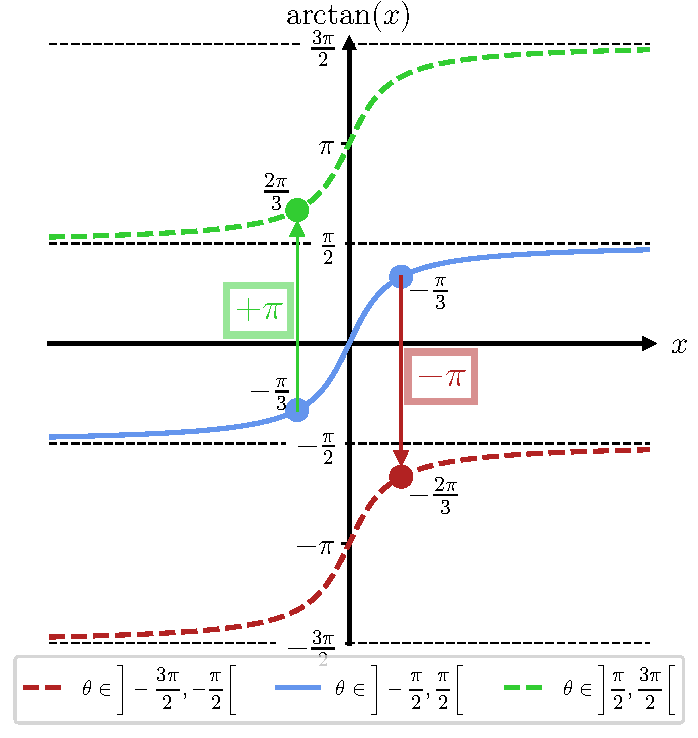
\includegraphics[width=0.85\linewidth]{fig_atan_prof}}
				}%
				\captionof{figure}{$\arctan(x)$}
				\\
				\sswitch{%
					{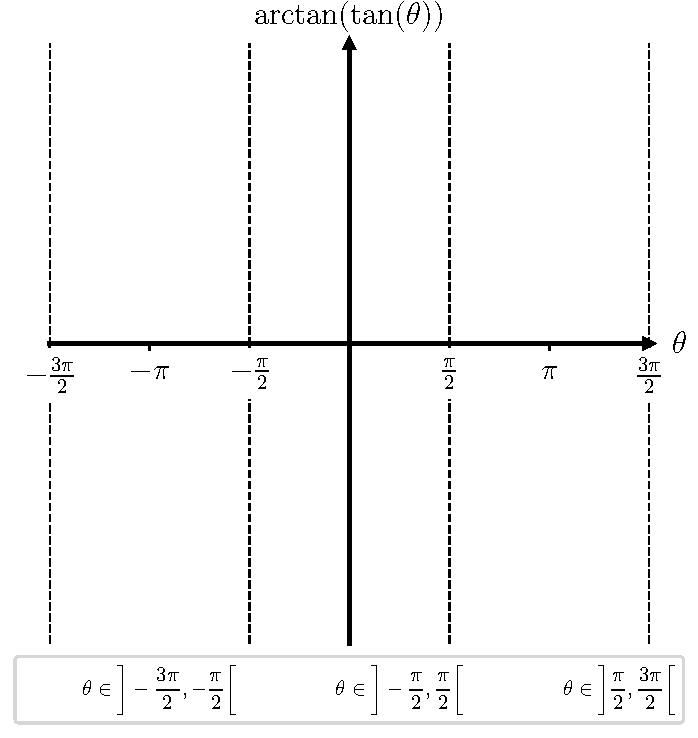
\includegraphics[width=0.85\linewidth]{fig_atantan_stud}}
				}{%
					{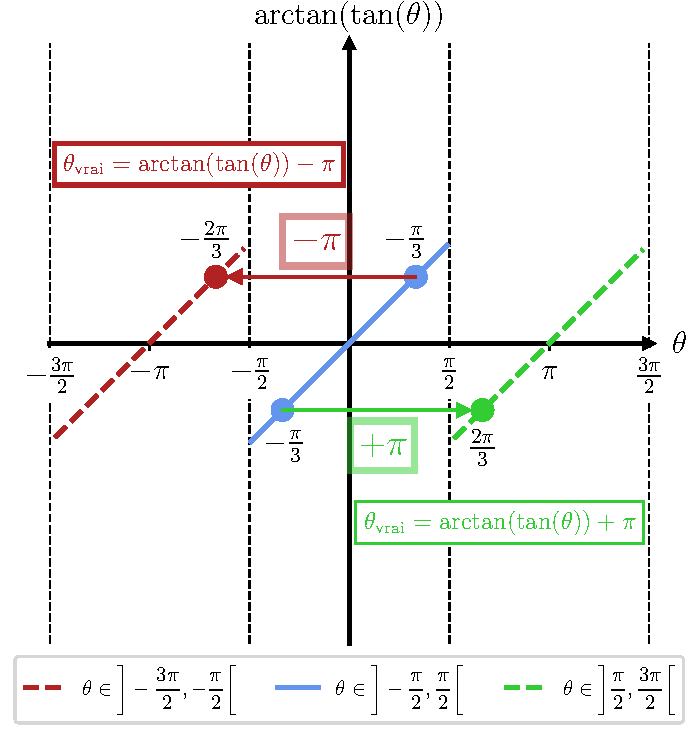
\includegraphics[width=0.85\linewidth]{fig_atantan_prof}}
				}%
				\captionof{figure}{$\arctan(\tan(\th))$}
				 &
				\sswitch{%
					{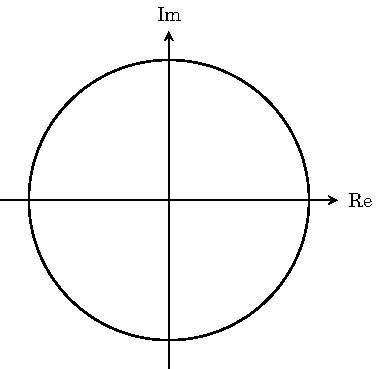
\includegraphics[width=0.85\linewidth]{fig_tan_xy_stud}}
				}{%
					{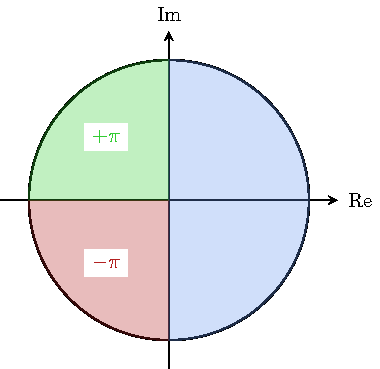
\includegraphics[width=0.85\linewidth]{fig_tan_xy_prof}}
				}%
				\captionof{figure}{Résumé}
			\end{tabularx}
		\end{center}
		Ainsi, \textbf{il faut vérifier} que $\f = \arg*{\Yu} \in
		\left] -\frac{\pi}{2} ; \frac{\pi}{2} \right[$ pour appliquer
	$\arctan(\tan(\th))$ sans souci. Pour cela, il suffit de vérifier que
		\psw{%
			\[
				\Re(\Yu) > 0
				\Lra
				\cos(\arg*{\Yu}) = \frac{\Re(\Yu)}{\abs{\Yu}} > 0
			\]
		}%
		Si ça n'est pas le cas, on détermine le signe de $\Im(\Yu)$. Alors, en
		utilisant également que $\tan(\th)$ soit $\pi$-périodique~:
	\begin{itemize}
		\item[m][32]
		      \begin{gather*}
			      \beforetext{$\DS\f = \arg*{\Yu} \in \left] \frac{\pi}{2} ; \pi \right] \Lra$}
			      \psw{%
				      \left\{
				      \begin{array}{ll}
					      \Re(\Yu) & < 0
					      \\
					      \Im(\Yu) & > 0
				      \end{array}
				      \right.
			      }%
			      \\\Ra
			      \psw{%
				      \arctan(\tan(\th-\pi)) = \th-\pi = \arctan(\tan(\th))
			      }%
			      \\\Lra
			      \psw{%
				      \boxed{\th = \arctan(\tan(\th)) + \pi}
			      }%
		      \end{gather*}
		\item[m][32]
		      \begin{gather*}
			      \beforetext{$\DS\f = \arg*{\Yu} \in \left[ -\pi ; -\frac{\pi}{2} \right[ \Lra$}
			      \psw{%
				      \left\{
				      \begin{array}{ll}
					      \Re(\Yu) & < 0
					      \\
					      \Im(\Yu) & < 0
				      \end{array}
				      \right.
			      }%
			      \\\Ra
			      \psw{%
				      \arctan(\tan(\th+\pi)) = \th+\pi = \arctan(\tan(\th))
			      }%
			      \\\Lra
			      \psw{%
				      \boxed{\th = \arctan(\tan(\th)) - \pi}
			      }%
		      \end{gather*}
	\end{itemize}
\end{tcb*}

\section{Circuits électriques en RSF}
Comme au début de l'année, nous nous plaçons toujours dans l'Approximation des
Régimes Quasi-Stationnaires (ARQS), c'est-à-dire que pour un circuit de taille
$L$ alimenté par une source sinusoïdale de fréquence $f$, on doit avoir
\fbox{$Lf \ll c$} avec $c$ la célérité de la lumière/des ondes
électromagnétiques.

\subsection{Lois de l'électrocinétique}
\subsubsection{Loi des nœuds en RSF}
\noindent
\begin{minipage}[t]{.48\linewidth}
	Soit un nœud où se rejoignent 5 branches. Dans l'ARQS, nous avions
	la relation ci-contre. En RSF, les intensités sont sinusoïdales \textbf{et
		de même pulsation} $\w$~: on aurait donc
\end{minipage}
\hfill
\begin{minipage}[t]{.48\linewidth}
	~
	\vspace{-50pt}
	\begin{center}
		\sswitch{%
			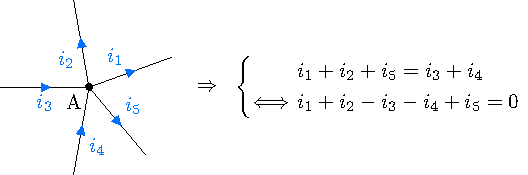
\includegraphics[width=\linewidth, draft=true]{ldn}
		}{%
			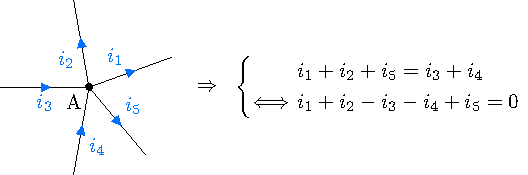
\includegraphics[width=\linewidth]{ldn}
		}%
		\captionof{figure}{Loi des nœuds}
	\end{center}
\end{minipage}
\[
	i_1(t) = I_1\cos(\wt+\f_1)
	\qet
	i_2(t) = I_2\cos(\wt+\f_2)
	\qet
	…
\]

\begin{tcb}(prop){Loi des nœuds en $\Cb$}
	Ainsi, en passant en complexes, on aura
	\psw{%
		\begin{gather*}
			\xul{i_1} + \xul{i_2} + \xul{i_5} = \xul{i_3} + \xul{i_4}
			\Lra
			\boxed{\xul{I_1} + \xul{I_2} + \xul{I_5} = \xul{I_3} + \xul{I_4}}\\
			\text{avec}\quad
			\xul{i_k} = I_k\exr^{\jj\f_k}\exr^{\jwt}
			\qet
			\xul{I_k} = I_k\exr^{\jj\f_k}
		\end{gather*}
	}%
	\vspace{-15pt}
	\begin{center}
		\textbf{On a donc la même relation avec les grandeurs et leurs amplitudes
			complexes}.
	\end{center}
\end{tcb}

\subsubsection{Loi des mailles}
% \begin{wrapfigure}[4]{R}{.5\linewidth}
% \vspace*{-30pt}
% \centering
% 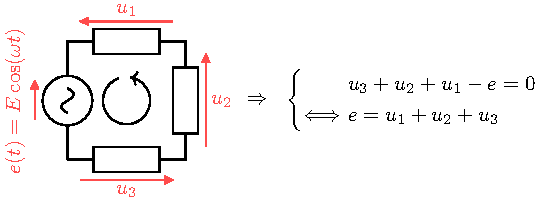
\includegraphics[width=\linewidth]{ldm_rsf}
% \end{wrapfigure}
\noindent
\begin{minipage}[t]{.48\linewidth}
	Soit une maille avec des dipôles quelconques, alimentée par une tension
	sinusoïdale $e(t) = E\cos(\wt)$. Dans l'ARQS, nous avions la relation
	ci-contre. En RSF, les tensions sont sinusoïdales \textbf{et de même
		pulsation} $\w$~: on aurait donc
\end{minipage}
\hfill
\begin{minipage}[t]{.48\linewidth}
	~
	\vspace{-40pt}
	\begin{center}
		\sswitch{%
			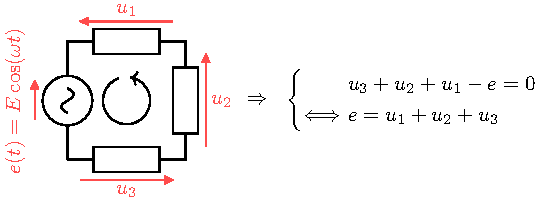
\includegraphics[width=\linewidth, draft=true]{ldm_rsf}
		}{%
			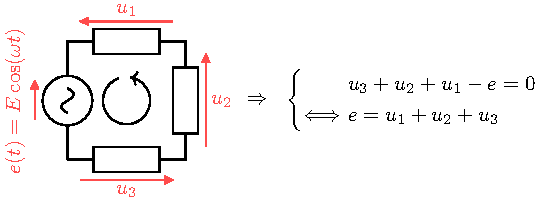
\includegraphics[width=\linewidth]{ldm_rsf}
		}%
		\captionof{figure}{Loi des mailles.}
	\end{center}
\end{minipage}
\[
	u_1(t) = U_1\cos(\wt+\f_1)
	\qet
	u_2(t) = U_2\cos(\wt+\f_2)
	\qet
	…
\]

\begin{tcb}(prop){Loi des mailles en $\Cb$}
	Ainsi, en passant en complexes, on aura
	\psw{%
		\begin{gather*}
			\eu = \xul{u_1} + \xul{u_2} + \xul{u_3}
			\Lra
			\boxed{\Eu = \xul{U_1} + \xul{U_2} + \xul{U_3}}\\
			\text{avec}\quad
			\xul{u_k} = U_k\exr^{\jj\f_k}\exr^{\jwt}
			\qet
			\xul{U_k} = U_k\exr^{\jj\f_k}
		\end{gather*}
	}%
	\vspace{-25pt}
	\begin{center}
		\textbf{On a donc la même relation avec les grandeurs et leurs amplitudes
			complexes}.
	\end{center}
\end{tcb}

\subsection{Exemple~: RC série en RSF}
\subsubsection{Présentation}
\begin{tcb}[sidebyside, righthand ratio=.4](defi){RC série en RSF}
	On s'intéresse au circuit suivant, composé d'une résistance et d'un
	condensateur $C$, alimentés par un GBF. On suppose une phase nulle pour le
	signal entrant~:
	\[
		e(t) = E_0 \cos(\wt)
		\qMath{ainsi}
		u_C(t) = U_C \cos(\wt+\f)
	\]
	Étant donné qu'on étudie le système en RSF, \textbf{on cherche l'amplitude
		complexe $\xul{U_C}$ de la tension du condensateur}.
	\tcblower
	\begin{center}
		\sswitch{%
			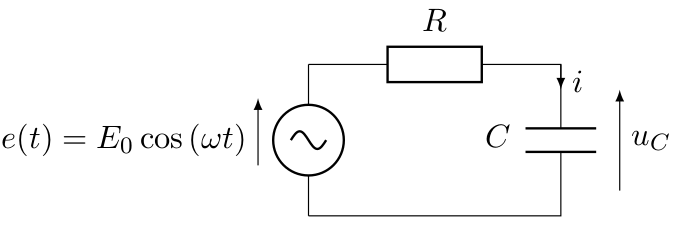
\includegraphics[width=\linewidth, draft=true]{rc_rsf}
		}{%
			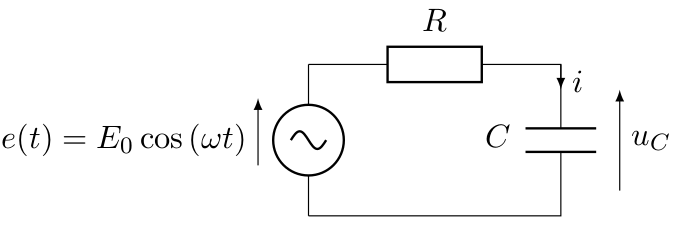
\includegraphics[width=\linewidth]{rc_rsf}
		}%
		\captionof{figure}{RC en RSF.}
	\end{center}
\end{tcb}

\subsubsection{Équation différentielle}
\begin{tcbraster}[raster equal height=rows, raster columns=2]
	\begin{tcb}(prop){Equ.\ diff.\ RC série}
		Dans un circuit RC série en RSF, $u_C(t)$ vérifie~:
		\[
			\psw{%
				\dv{u_C}{t} + \frac{1}{\tau} u_C = \frac{1}{\tau} E_0 \cos(\wt)
			}%
			\qav
			\psw{%
				\tau = RC
			}%
		\]
	\end{tcb}
	\begin{tcb}(demo)'r'{Equ.\ diff.\ RC}
		\vspace{-15pt}
		\psw{%
			\begin{DispWithArrows*}[fleqn, mathindent=-5pt]
				u_R + u_C &= e(t)
				\Arrow{$u_R = Ri$}
				\\\Lra
				Ri + u_C &= e(t)
				\Arrow{$i = C \dv{u_C}{t}$}
				\\\Lra
				RC \dv{u_C}{t} + u_C &= e(t)
				\Arrow{Forme can.}
				\\\Lra
				\Aboxed{%
					\dv{u_C}{t} + \frac{1}{\tau}u_C &= \frac{1}{\tau}E_0\cos(\wt)
				}%
			\end{DispWithArrows*}
		}%
		\vspace{-15pt}
	\end{tcb}
\end{tcbraster}

\subsubsection{Solution}

\begin{tcb*}[sidebyside, righthand ratio=.6](prop){$u_C(t)$ en RSF}
	% L'amplitude complexe de la tension aux bornes d'un condensateur en RSF est
	% \[
	%   \psw{%
	%     \xul{U_C} = \frac{E_0}{1+ \jj RC\w}
	%   }%
	% \]
	Ainsi, la tension réelle s'écrit
	\begin{gather*}
		\boxed{u_C(t) = U_C \cos(\wt + \f)} \qav
		\\
		\left\{
		\psw{%
			\begin{array}{ll}
				U_C & = \DS\frac{E_0}{\sqrt{1+ (RC\w)^2}}
				\\[2em]
				\f  & - \arctan(RC\w)
			\end{array}
		}%
		\right.
	\end{gather*}
	\tcblower
	\noindent
	\begin{minipage}[t]{.48\linewidth}
		\vspace{0pt}
		\begin{center}
			\sswitch{%
				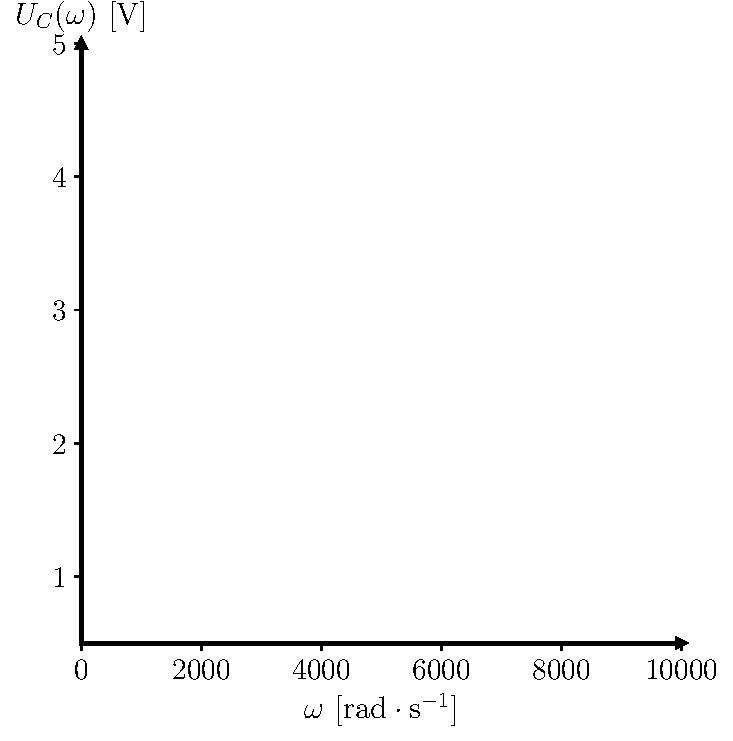
\includegraphics[width=\linewidth]{Ucw_ampl_stud}
			}{%
				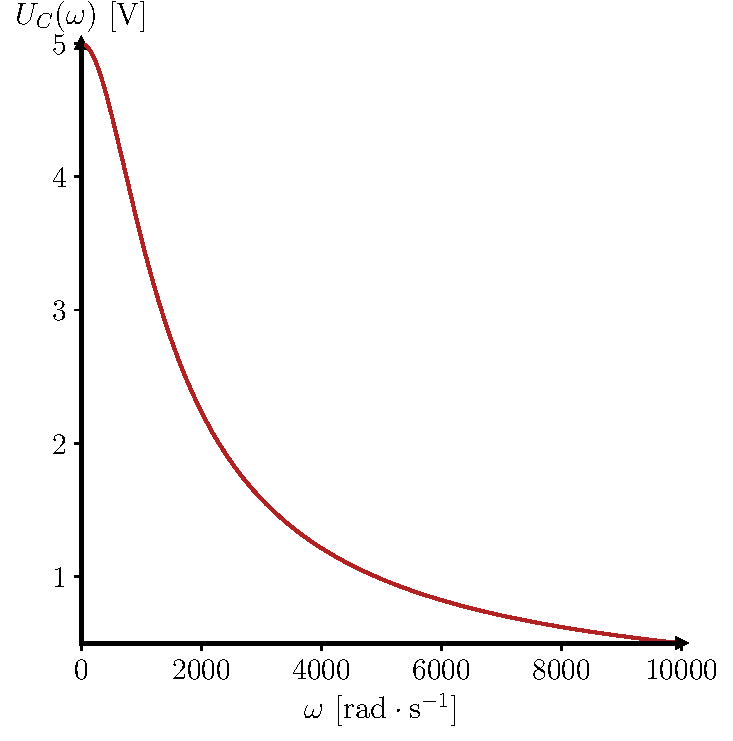
\includegraphics[width=\linewidth]{Ucw_ampl_prof}
			}%
			\captionof{figure}{}
		\end{center}
	\end{minipage}
	\hfill
	\begin{minipage}[t]{.48\linewidth}
		\vspace{0pt}
		\begin{center}
			\sswitch{%
				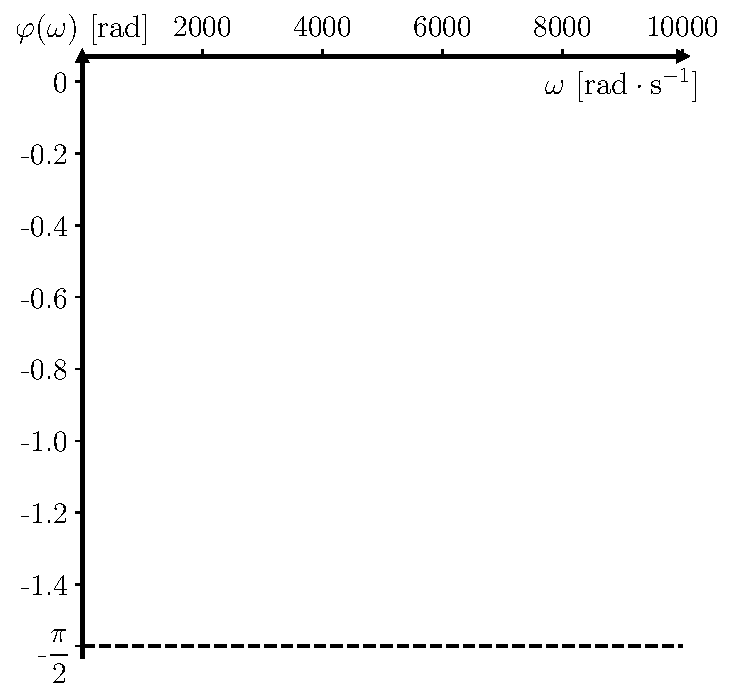
\includegraphics[width=\linewidth]{Ucw_arg_stud}
			}{%
				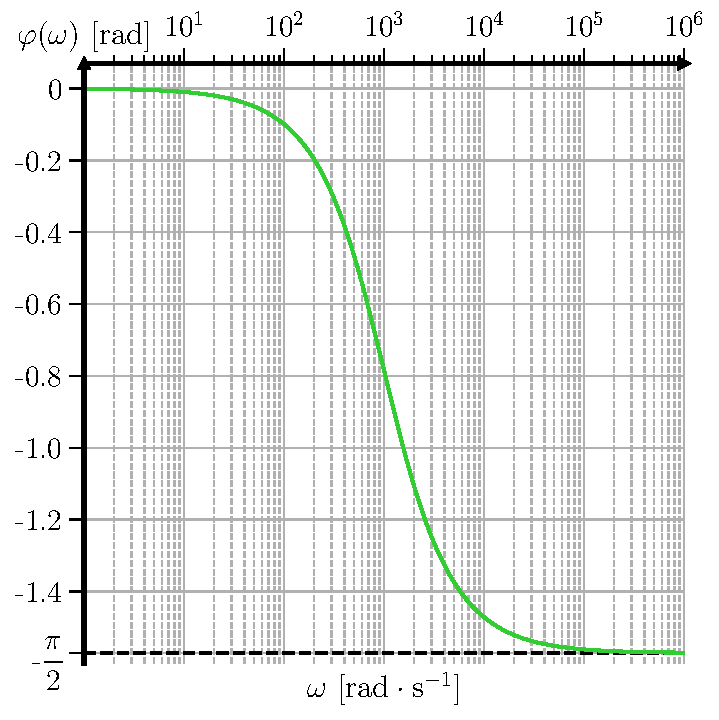
\includegraphics[width=\linewidth]{Ucw_arg_prof}
			}%
			\captionof{figure}{}
		\end{center}
	\end{minipage}
\end{tcb*}

% Résoudre cette équation différentielle demande comme précédemment de trouver la
% solution homogène et la solution particulière. La solution homogène est la
% solution de
% \begin{gather*}
% 	\dv{u_{C,h}}{t} + \frac{1}{\tau}u_{C,h} = 0
% 	\Ra
% 	u_{C,h}(t) = A\exp \left( - \frac{t}{\tau} \right)
% \end{gather*}
% Pour la solution particulière, \textbf{on admet} qu'elle est de la forme
% \begin{gather*}
% 	\psw{%
% 		u_{C,p}(t) = U\cos(\wt + \f)
% 	}%
% \end{gather*}
% ce qui donne une solution générale
% \psw{%
% 	\[\boxed{u_C(t) = A\exp \left( - \frac{t}{\tau} \right) + U\cos(\wt + \f)}\]
% }
% \vspace{-15pt}
% \begin{tcb}[label=ror:CIounon](impo){Important}
% 	$K$ dépend des conditions initiales, mais
% 	\smallbreak \centering\large
% 	$U$ et $\f$ dépendent du circuit (ici, $R$, $C$, $\w$ et $E_0$).
% \end{tcb}
%
% \subsection{Réponse d'un système en RSF}
% En supposant le régime permanent établi (définition du RSF), on a donc~:
% \begin{tcb}[label=prop:sortiersf](ror){Forme de la réponse d'un système en RSF}
% 	\psw{%
% 		Pour un signal d'entrée
% 		\[
% 			e(t) = E_0 \cos(\wt)
% 			\quad(\text{ou}\quad
% 			\eta(t) = \eta_0\cos(\wt))
% 		\]
% 		les différentes tensions et intensités dans le circuit oscilleront \textbf{à
% 			la même pulsation $\w$}, et seront de la forme
% 		\[
% 			u(t) = U\cos(\wt+\f_u)
% 			\qet
% 			i(t) = I\cos(\wt+\f_i)
% 		\]
% 		où $U,I$ et $\f_{u,i}$ sont deux constantes dépendant du système et de
% 		l'excitation $\w$.
% 	}%
% \end{tcb}
% \begin{tcb}[cnt, bld](impl)<lfnt>{}
% 	L'objectif de ce chapitre est de donc de savoir déterminer $U$ et $\f$.
% \end{tcb}
% \subsection{Passage en complexes}
% Une méthode de résolution est d'introduire la formule $U\cos(\wt+\f)$ dans
% l'équation différentielle et de rechercher $U$ et $\f$. Si c'est possible, c'est
% très calculatoire (cf.\ cours de maths). L'utilisation des nombres complexes
% permet de réduire drastiquement cette difficulté.
%
% \begin{tcb}(tool){Méthode}
% 	Pour cela, on remplace $u(t)$ et $e(t)$ par leurs formes complexes~:
% 	\psw{%
% 		\begin{gather*}
% 			\xul{u_C} = \Uu\exr^{\jwt}
% 			\qavec
% 			\Uu = U\exr^{\jj\f}
% 			\qet
% 			\eu = E_0\exr^{\jwt}
% 		\end{gather*}
% 	}%
% 	Pour revenir aux valeurs réelles après calcul, on prendra donc
% 	\psw{%
% 		\begin{gather*}
% 			U_C = \abs{\xul{U_C}}
% 			\qet
% 			\f = \arg*{\xul{U_C}}
% 		\end{gather*}
% 	}%
% \end{tcb}

\begin{tcb*}(demo){Solution RC en RSF}
	En RSF, $u_C(t)$ prend la forme de l'entrée, donc on
	cherche $u_C(t) = U_C \cos(\wt+\f)$. Ainsi, à partir de l'équation
	différentielle, on passe toutes les grandeurs en complexes~:
	\smallbreak
	\begin{isd}[interior hidden, sidebyside align=top](demo)
		\tcbsubtitle{\fatbox{\textbf{Amplitude complexe}}}
		\psw{%
			\begin{DispWithArrows*}[fleqn, mathindent=-2pt, groups]
				\dv{\xul{u_C}}{t} + \frac{\xul{u_C}}{\tau}    & = \frac{\eu}{\tau}
				\Arrow{$\uu_C = \Uu_C\exr^{\jwt}$\\et $\dv{\yu}{t} = \jw \yu(t)$}
				\\\Lra
				\jw\xul{U_C}\cancel{\exr^{\jwt}} +
				\frac{\xul{U_C}\cancel{\exr^{\jwt}}}{RC}                          & =
				\frac{E_0\cancel{\exr^{\jwt}}}{RC}
				\Arrow{On factorise}
				\\\Lra
				\xul{U_C} \left( RC\jw + 1 \right) & = E_0
				\Arrow[new-group]{On isole}
				\\\Lra
				\Aboxed{
					\xul{U_C}                          & = \frac{E_0}{1 + \jj RC\w}}
			\end{DispWithArrows*}
		}%
		\vspace{-15pt}
		\tcblower
		\tcbsubtitle{\fatbox{\textbf{Module}}}
		\psw{%
			\begin{align*}
				U_C
				= \abs{\xul{U_C}}
				    & = \abs{\frac{E_0}{1 + \jj RC\w}}
				\\\Lra
				U_C & =
				= \frac{\abs{E_0}}{\abs{1 + \jj RC\w}}
				\\\Lra
				\Aboxed{
				U_C & = \frac{E_0}{\sqrt{1+(RC\w)^2}}
				}%
			\end{align*}
		}%
		\vspace{-15pt}
	\end{isd}
	\tcbsubtitle{\fatbox{\textbf{Argument}}}
	\vspace{-15pt}
	\psw{%
		\begin{gather*}
			\f
			= \arg*{ \frac{E_0}{1+\jj RC\w} }%
			= \underbracket{\arg*{E_0}}_{=0} - \arg{1+\jj RC\w}
			\\\Ra
			\tan(\f)
			= - \tan\/(\arg{\underbracket[1pt]{1}_{\mathclap{\Re > 0}}+\jj RC\w})
			= - \frac{RC\w}{1}
		\end{gather*}
		Comme on a $\Re(\arg{1+\jj RC\w}) > 0$, on applique simplement $\arctan(\cdot)$~:
		\[\boxed{\f = -\arctan(RC\w)}\]
	}%
	\vspace{-15pt}
\end{tcb*}

% D'une manière générale, on utilisera l'expression de la tangente d'un
% argument \textbf{avant} de voir si on peut prendre l'arctangente de la
% tangente.
% \begin{tcb}(impo){Attention}
% 	Ça peut être une réponse acceptable dans certaines conditions, mais bien souvent
% 	on souhaite exprimer la phase directement. Dans ce cas, il faut faire attention
% 	au fait que
% 	\[
% 	\arctan(\tan(\theta)) = \theta
% 	\Lra
% 	\theta \in \left] - \frac{\pi}{2}\,; \frac{\pi}{2} \right[
% 		\]
% 		Une manière de s'assurer de l'appartenance de $\theta$ à cet intervalle, il
% 		suffit de regarder la \textbf{partie réelle} de l'argument, ou bien son
% 		cosinus~: s'il est positif, alors on a en effet $\theta \in \left] -
% 	\frac{\pi}{2}\,; \frac{\pi}{2} \right[$. Ici,
% 		\begin{gather*}
% 			\cos(\arg*{\f})
% 			= \frac{\Re(\arg*{\f})}{\abs{\zu}}
% 			= \frac{1}{\sqrt{1 + (RC\w)^2}} > 0
% 		\end{gather*}
% 		donc on peut bien dire que $\arctan\tan(\f) = \f$.
% 		\smallbreak
% 		Si ça n'est pas le cas, il faut ajouter ou soustraire $\pi$ à l'argument.
% \end{tcb}
% % TODO: graphiques pour expliquer si on ajoute ou soustrait \pi.
%
% \begin{tcb}(prop){Résultat}
% 	La solution particulière est
% 	\psw{%
% 		\begin{gather*}
% 			\boxed{u_C (t) = U_C\cos(\wt + \f)}
% 			\\\text{avec}\\
% 			\boxed{U_C = \frac{E_0}{\sqrt{1+(RC\w)^2}}}
% 			\qet
% 			\boxed{\f = -\arctan(RC\w)}
% 		\end{gather*}
% 	}%
% \end{tcb}
%
% \begin{tcb}(rema)<lfnt>{Remarque~: dépendance en $\w$}
% 	Comme on l'a vu, le signal de sortie sera à la même pulsation que le signal
% 	d'entrée, mais par cet exemple du circuit RC on note que la phase et
% 	l'amplitude \textbf{dépendent de la pulsation}.
% \end{tcb}

% \begin{tcb}*(expe)<itc>"trans"{Transition}
% 	À partir de cet exemple, est-ce qu'on peut étendre l'utilisation des
% 	complexes pour le RSF aux lois de bases de l'électrocinétique~?
% \end{tcb}

\subsection{Impédance et admittance complexes d'un dipôle passif}
\subsubsection{Définition}
En complexes, pour chaque dipôle on aura
\begin{align*}
	\psw{%
		u(t) = U\cos(\wt+\f_u)
	}%
	 & \qet
	\psw{%
		i(t) = I\cos(\wt+\f_i)
	}%
	\\
	\beforetext{$\Longrightarrow$}
	\psw{%
		\uu(t) = U\exr^{\jj(\wt+\f_u)} = U\exr^{\jj\f_u}\exr^{\jwt} =
		\Uu\exr^{\jwt}
	}%
	 & \qet
	\psw{%
		\iu(t) = I\exr^{\jj(\wt+\f_i)} = I\exr^{\jj\f_i}\exr^{\jwt} =
		\Iu\exr^{\jwt}
	}%
\end{align*}
Ainsi, on peut aisément exprimer une relation courant-tension pour un dipôle
complexe, sous la forme classique $U = RI$ mais en complexes. On peut
tout à fait calculer $\frac{\uu}{\iu}$ pour avoir une proportionnalité
entre les deux~: on appelle cette constante l'\textbf{impédance}, notée
$\Zu$, et on a donc la \textbf{loi d'Ohm complexe}~:

\begin{tcb*}[sidebyside](defi){Impédance complexe}
	\tcbsubtitle{\fatbox{Loi d'Ohm complexe}}
	\psw{%
		\begin{gather*}
			\uu(t) = \Zu\iu(t)
			\Lra
			\boxed{\Uu = \Zu\times\Iu}\\
			\Rightarrow
			\Zu\quad\text{homogène à une résistance}
		\end{gather*}
	}%
	\tcblower
	\begin{center}
		\sswitch{%
			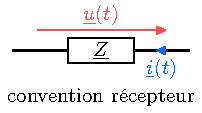
\includegraphics[width=.5\linewidth, draft=true]{zdef}
		}{%
			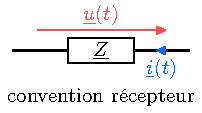
\includegraphics[width=.5\linewidth]{zdef}
		}%
		\captionof{figure}{Représentation d'une impédance complexe}
	\end{center}
\end{tcb*}

En tant que complexe, on peut prendre son module et son argument~:
\begin{tcb}(prop){Impédance complexe}
	\begin{itemize}
		\item Son module $Z = \abs{\Zu}$ est égal au rapport de
		      l'amplitude de $u$ sur celle de $i$~:
		      \psw{%
			      \[
				      \boxed{ \abs{\Zu}
					      = \frac{\abs{\uu}}{\abs{\iu}}
					      = \frac{U}{I}
				      }%
			      \]
		      }%
		\item Son argument $\arg*{\Zu}$ est égal à la différence de phase entre
		      $\uu$ et $\iu$ (aussi appelée \textbf{déphasage}, voir Section
		      ultérieure)~:
		      \psw{%
			      \[
				      \boxed{\arg*{\Zu}
					      = \arg*{ \frac{\uu}{\iu} }%
					      = \f_u - \f_i}
			      \]
		      }%
	\end{itemize}
\end{tcb}


\begin{tcb}(defi){Admittance}
	Assez naturellement, comme on avait la conductance égale à l'inverse d'une
	résistance, on peut définir l'inverse d'une impédance~: c'est
	l'\textbf{admittance complexe} $\Yu$~:
	\psw{%
		\[
			\boxed{\Yu
				= \frac{1}{\Zu} \Rightarrow \Iu
				= \Yu\times\Uu}
		\]
	}%
\end{tcb}

\subsubsection{Impédances de bases}

Pour trouver les impédances des dipôles de base, on utilise leurs relations
courant-tension qu'on convertit en complexes, \textbf{en se souvenant de dériver
	en complexes équivaut à multiplier par $\jw$}.

\begin{tcb*}[tabularx={l|Y|Y|Y}](defi)
	{Impédances des dipôles de base}
	&
	\vspace{8pt}
	\textbf{Résistance} &
	\vspace{8pt}
	\textbf{Inductance} &
	\vspace{8pt}
	\textbf{Capacité}
	\\\hline
	\rotatebox[origin=c]{90}{Schéma} &
	\sswitch{%
		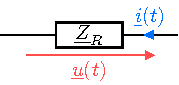
\includegraphics[height=2cm, draft=true]{zr}
	}{%
		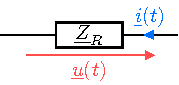
\includegraphics[height=2cm]{zr}
	}%
	\captionof{figure}{$\xul{Z_R}$}
	&
	\sswitch{%
		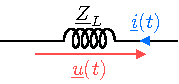
\includegraphics[height=2cm, draft=true]{zl}
	}{%
		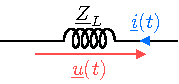
\includegraphics[height=2cm]{zl}
	}%
	\captionof{figure}{$\xul{Z_L}$}
	&
	\sswitch{%
		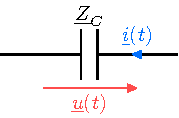
\includegraphics[height=2cm, draft=true]{zc}
	}{%
		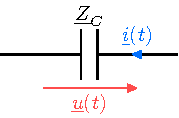
\includegraphics[height=2cm]{zc}
	}%
	\captionof{figure}{$\xul{Z_C}$}
	\\\hline
	\rotatebox[origin=c]{90}{Démonstration} &
	\psw{%
		$\begin{aligned}
				u(t)          & = Ri(t)   \\
				\Lra
				\uu(t)        & = R\iu(t) \\
				\Lra
				\Aboxed{\Zu_R & = R}
			\end{aligned}$
	}%
	&
	\psw{%
		$\begin{aligned}
				u(t)          & = L\dv{i}{t}    \\
				\Lra
				\uu(t)        & = \jj L\w\iu(t) \\
				\Lra
				\Aboxed{\Zu_L & = \jj L\w}
			\end{aligned}$
	}%
	&
	\psw{%
		$\begin{aligned}
				i(t)          & = C\dv{u}{t}         \\
				\Lra
				\iu(t)        & = C\jwt\uu(t)        \\
				\Lra
				\Aboxed{\Zu_C & = \frac{1}{\jj C\w}}
			\end{aligned}$
	}%
	\\\hline
\end{tcb*}

\subsubsection{Comportements limites}
Ainsi, la résistance ne change pas d'expression entre les réels et les
complexes, alors que les bobines et condensateurs ont des caractéristiques
complexes différentes. En plus de ça, leurs impédances \textbf{dépendent} de
$\w$~: on peut notamment étudier deux cas limites, quand $\w\rightarrow0$ et
$\w\rightarrow+\infty$~:
\begin{tcb*}[tabularx*={\renewcommand{\arraystretch}{1.5}}{l|Y|Y}](prop){Dipôles
			équivalents aux limites}
	&
	$\w\rightarrow0$ &
	$\w\rightarrow+\infty$
	\\\hline
	\rotatebox[origin=c]{90}{Bobine} &
	\psw{%
		$\abs{\Zu_L} = L\w \underset{\w\rightarrow0}{\rightarrow}0$
	}%
	\smallbreak
	\sswitch{%
		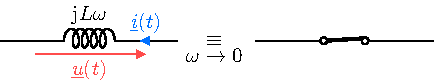
\includegraphics[width=\linewidth, draft=true]{zlwa}
	}{%
		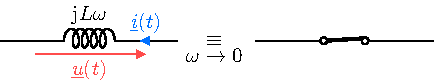
\includegraphics[width=\linewidth]{zlwa}
	}%
	\vspace{-15pt}
	&
	\psw{%
		$\abs{\Zu_L} = L\w \underset{\w\rightarrow+\infty}{\rightarrow}+\infty$
	}%
	\smallbreak
	\sswitch{%
		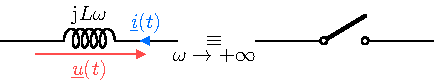
\includegraphics[width=\linewidth, draft=true]{zlwi}
	}{%
		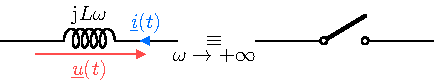
\includegraphics[width=\linewidth]{zlwi}
	}%
	\vspace{-15pt}
	\\\hline
	\rotatebox[origin=c]{90}{Condensateur} &
	\psw{%
		$\abs{\Zu_C} = 1/(C\w) \underset{\w\rightarrow0}{\rightarrow}+\infty$
	}%
	\smallbreak
	\sswitch{%
		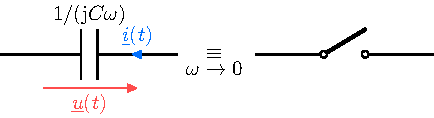
\includegraphics[width=\linewidth, draft=true]{zcwa}
	}{%
		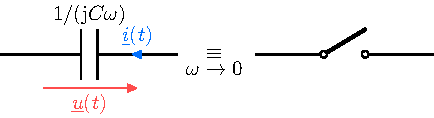
\includegraphics[width=\linewidth]{zcwa}
	}%
	\vspace{-15pt}
	&
	\psw{%
		$\abs{\Zu_C} = 1/(C\w) \underset{\w\rightarrow+\infty}{\rightarrow}0$
	}%
	\smallbreak
	\sswitch{%
		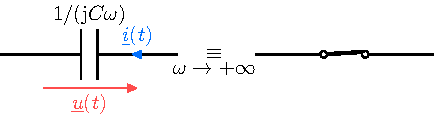
\includegraphics[width=\linewidth, draft=true]{zcwi}
	}{%
		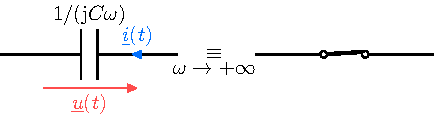
\includegraphics[width=\linewidth]{zcwi}
	}%
	\vspace{-15pt}
\end{tcb*}
% En effet, l'impédance étant homogène à une résistance, on peut rendre équivalent
% le fait d'avoir une impédance infinie et d'avoir une «~résistance~» infinie,
% c'est-à-dire un interrupteur ouvert, qui ne laisse pas passer le courant. À
% l'inverse, une résistance nulle laisse passer le courant sans résistance, comme
% un fil.

% \vspace{-15pt}
\subsection{Associations d'impédances et ponts diviseurs}
Enfin, comme la relation courant-tension avec l'impédance complexe est analogue
à celle d'une résistance, on peut facilement démontrer que les associations
d'impédances suivent les associations de résistances, et qu'on peut donc
appliquer les ponts diviseurs de tension et de courant comme si on n'avait que
des résistances.
% \vspace{-15pt}
\begin{tcb}[tabularx={l|Y|Y}](ror){Associations d'impédances}
	&
	\vspace{8pt}
	\textbf{Schéma} &
	\textbf{Relations}
	\\\hline
	\rotatebox[origin=c]{90}{\textbf{En série}} &
	\sswitch{%
		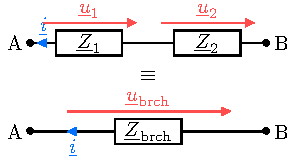
\includegraphics[width=\linewidth, draft=true]{zserie}
	}{%
		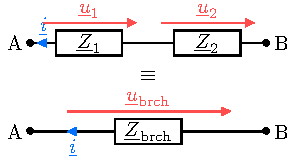
\includegraphics[width=\linewidth]{zserie}
	}%
	\vspace{-15pt}
	&
	\begin{itemize}
		\item[b]{Impédance équivalente} :
		      \psw{%
			      \[\Zu\ind{eq} = \Zu_1 + \Zu_2\]
		      }%
		      \vspace{-15pt}
		\item[b]{Diviseur de tension} :
		      \psw{%
			      \[\xul{u_k} = \frac{\Zu_k}{\Zu_{\rm
						      brch}}\uu\ind{brch}\]
		      }%
		      \vspace{-15pt}
	\end{itemize}
	\\\hline
	\rotatebox[origin=c]{90}{\textbf{En parallèle}} &
	\sswitch{%
		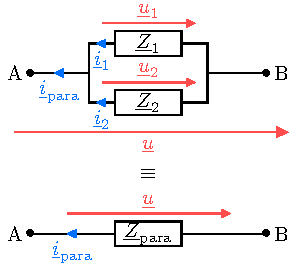
\includegraphics[width=.7\linewidth, draft=true]{zpara}
	}{%
		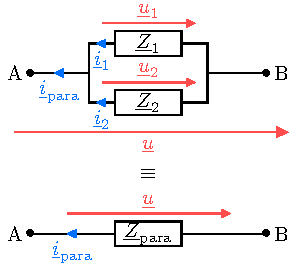
\includegraphics[width=.7\linewidth]{zpara}
	}%
	\vspace{-15pt}
	&
	\begin{itemize}
		\item[b]{Dipôle équivalent} :
		      \psw{%
			      \begin{gather*}
				      \Yu\ind{eq} = \Yu_1 + \Yu_2
				      \\\Lra
				      \frac{1}{\Zu\ind{eq}} = \frac{1}{\Zu_1} + \frac{1}{\Zu_2}
				      \Lra
				      \Zu\ind{eq} = \frac{\Zu_1\Zu_2}{\Zu_1+\Zu_2}
			      \end{gather*}
		      }%
		      \vspace{-15pt}
		\item[b]{Diviseur de courant} :
		      \psw{%
			      \begin{gather*}
				      \xul{i_k} = \frac{\Yu_k}{\Yu_{\rm para}}\iu\ind{para}
				      \Lra
				      \xul{i_k} = \frac{\Zu_{\rm para}}{\Zu_k}\iu\ind{para}\\
				      % \Lra
				      % \xul{i_{\fbox{1}}} = \frac{\Zu_{\fbox{2}}}{\Zu_1 + \Zu_2}\iu
			      \end{gather*}
		      }%
		      \vspace{-30pt}
	\end{itemize}
\end{tcb}

\subsection{Exercices bilan}
\begin{tcb}[sidebyside, righthand ratio=.7](appl)<lftt>{Association d'impédances}
	Quelle est l'impédance de l'association suivante~?
	\begin{center}
		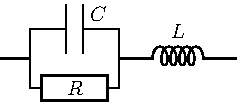
\includegraphics[width=\linewidth]{exo_zeq}
	\end{center}
	\tcblower
	\psw{%
		L'association en parallèle donne
		$\frac{\Zu_C\Zu_R}{\Zu_C+\Zu_R}$, et on ajoute $\Zu_L$ à
		celle-ci~:
		\begin{gather*}
			\Zu\ind{eq}
			= \frac{\dfrac{1}{\jj C\w}\times R}{\dfrac{1}{\jj C\w} + R}
			+ \jj L\w
			\Lra
			\boxed{
				\Zu\ind{eq} = \frac{R}{1+\jj RC\w} + \jj L\w}
		\end{gather*}
	}%
	\vspace{-15pt}
\end{tcb}

\begin{tcb}[valign=top](appl)<lftt>{RLC parallèle en RSF}
	\begin{isd}[sidebyside align=center, righthand ratio=.4]
		Soit le circuit suivant, avec une entrée sinusoïdale $e(t) = E\cos(\wt)$.
		Exprimer l'amplitude complexe $\Uu_C$ associée à la tension $u_C$ en
		fonction de $R$, $L$, $C$ et $\w$.
		\tcblower
		\begin{center}
			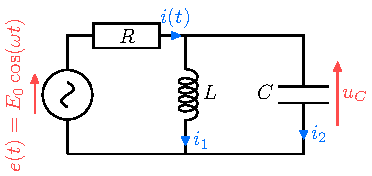
\includegraphics[width=\linewidth]{rlc_r-s-LC-parr}
		\end{center}
	\end{isd}
	\tcblower
	\psw{%
		S'il n'y avait pas l'inductance, on pourrait facilement utiliser un pont
		diviseur de tension pour exprimer $\uu_C$ en fonction de $\eu$,
		$\Zu_R$ et $\Zu_C$. Pour se ramener à la situation du pont diviseur de
		tension, on détermine donc une première impédance équivalente issue de
		l'association en parallèle de $L$ et $C$, après les avoir converties en
		complexes~:
		\vspace{-15pt}
		\begin{center}
			\sswitch{%
				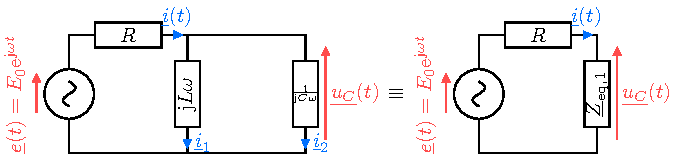
\includegraphics[width=\linewidth, draft=true]{rlc_r-s-LC-parr_cplx}
			}{%
				\includegraphics[width=\linewidth]{rlc_r-s-LC-parr_cplx}
			}%
		\end{center}
		On peut déterminer $\Zu_{\eql, 1}$ avec les admittances $\Yu_L = 1/\jj
			L \w$ et $\Yu_C = \jj C\w$, et utiliser le pont diviseur de tension
		directement avec l'amplitude complexe~: $\Uu_C =
			\frac{\Zu_{\eql,1}}{\Zu_{\eql,1}+\Zu_R}E_0$. Ainsi,
		\begin{gather*}
			\Uu_C = \frac{\dfrac{1}{%
					\psw[orange]{\cancel{\dfrac{1}{\jj L\w} + \jj C\w}}}}
			{\dfrac{1}{\psw[orange]{\cancel{\dfrac{1}{\jj L\w} + \jj C\w}}}
				+ R\psw[orange]{(…)}}E_0
			\times \psw[orange]{
				\frac{\jj C\w + \dfrac{1}{\jj L\w}}{\jj C\w + \dfrac{1}{\jj L\w}}}
			\Lra
			\Uu_C = \frac{1}{1 + \jj RC\w + \dfrac{R}{\jj L\w}}E_0\\
			\Lra
			\boxed{
				\Uu_C = \frac{E_0}{1 + \jj \left( RC\w - \dfrac{R}{L\w} \right)}
			}%
		\end{gather*}
		où on a simplifié la fraction en multipliant par le terme orange d'abord,
		puis en utilisant que $1/\jj = -\jj$.
	}%
\end{tcb}

\subsection{Résumé}

\begin{tcb}(ror){Résumé méthode}
	Un système soumis à une excitation sinusoïdale du type $e(t) = E_0\cos(\wt)$
	se comporte de la manière suivante~:
	\begin{itemize}
		\item On observe un court régime transitoire dû à la solution homogène de
		      l'ED ($A\exr^{-t/\tau}$ pour ordre 1, pseudo-périodique ou apériodique
		      pour l'ordre 2)~;
		\item Après ce régime, on obtient la solution particulière~:
		      \[
			      x(t) = X\cos(\wt+\f_X)
		      \]
		      avec $\w$ la \textbf{pulsation d'entrée}, $X$ et $\f_X$  définies
		      \textbf{par le système} (et non pas des conditions initiales).
		\item Pour trouver ces valeurs, on définit~:
		      \begin{itemize}
			      \item \leftcenters{l'entrée complexe~:}
			            {\psw{$\eu(t) = E_0\exr^{\jwt}$}}
			            \vspace{-10pt}
			      \item \leftcenters{les signaux de sortie complexes~:}
			            {\psw{$\xu(t) = X\exr^{\jj(\wt+\f_X)}$~;}}
			            \vspace{-10pt}
			      \item \leftcenters{les amplitudes complexes~:}
			            {\psw{$\Xu = X\exr^{\jj\f_X}
						            \Ra
						            \xu(t) = \Xu\exr^{\jwt}$~;}}
			            \vspace{-5pt}
			      \item On retrouve les grandeurs réelles en en prenant le module et
			            la phase~:
			            \psw{%
				            \[
					            \boxed{X = \abs{\Xu}}
					            \qet
					            \boxed{\f_X = \arg*{\Xu}}
				            \]
			            }%
			            \vspace{-15pt}
		      \end{itemize}
	\end{itemize}
\end{tcb}

\section{Mesure de déphasages}
\subsection{Définition}
\begin{tcb}(defi){Déphasage}
	Pour deux signaux sinusoïdaux \textbf{de mêmes fréquences} $s_1(t) =
		S_1\cos(\wt+\f_1)$ et $s_2(t) = S_2\cos(\wt+\f_2)$, on définit le
	\textbf{déphasage} entre $s_2$ et $s_1$ comme étant la \textbf{différence de
		leurs phases instantanées}~:
	\psw{%
		\[
			\D\f_{2/1} = (\wt + \f_2) - (\wt+\f_1)
			\Lra
			\boxed{\D\f_{2/1} = \f_2 - \f_1}
		\]
	}%
	\vspace{-15pt}
\end{tcb}
% \begin{tcb}(rapp){}
% 	Étant donné que les sorties en RSF ont la même pulsation que l'entrée, on ne
% 	s'intéressera qu'à des signaux de même pulsation/fréquence.
% \end{tcb}

\subsection{Lecture d'un déphasage}

\noindent
\begin{minipage}{0.65\linewidth}
	Le déphasage $\D\f_{2/1} = \f_2 - \f_1$ est lié au \textbf{retard temporel}
	$\D{t}_{2/1} = t_2 - t_1$ du signal $s_2$ par rapport au signal $s_1$~: on a
	\psw{%
		\[\boxed{\abs{\D\f_{2/1}} = \w \abs{\D{t}_{2/1}}}\]
	}%
	Dans ce cas, le déphasage obtenu est entre $-\pi$ et $+\pi$. On définit~:
	\begin{itemize}
		\item \psw{%
			      $\D\f_{2/1} > 0 \Rightarrow s_2$ est en avance sur $s_1$~;
		      }%
		\item \psw{%
			      $\D\f_{2/1} < 0 \Rightarrow s_2$ est en retard sur $s_1$.
		      }%
	\end{itemize}
\end{minipage}
\hfill
\begin{minipage}{0.30\linewidth}
	\vspace{-15pt}
	\begin{center}
		\sswitch{%
			\includegraphics[width=\linewidth, draft=true]{dfeqr}
		}{%
			\includegraphics[width=\linewidth]{dfeqr}
		}%
		\captionof{figure}{Déphasage}
	\end{center}
\end{minipage}

Le principe est de mesurer la différence de temps entre les deux moments les
plus proches tels que les deux signaux s'annulent \textbf{avec la même pente}.
% Par construction, la pulsation représente une vitesse angulaire, c'est pourquoi
% on a $\w = 2\pi/T$ comme $v = d/t$ en mécanique. On trouve donc naturellement la
% relation entre $\D\f_{2/1}$ et $\D{t}_{2/1}$.

\subsection{Valeurs particulières}
\begin{tcb}[sidebyside, righthand ratio=.3](defi){Signaux en phase}
	Deux signaux sont \textbf{en phase} si leur \textbf{déphasage est nul}
	(modulo $2\pi$)~:
	\psw{%
		\[
			\D\f \equiv 0\quad[2\pi]
			\Lra
			\boxed{\D\f = 2p\pi} \quad p \in \Zb
		\]
	}%
	Les signaux passent par leurs valeurs maximales et minimales aux mêmes
	instants, et s'annulent simultanément.
	\tcblower
	\begin{center}
		\sswitch{%
			\includegraphics[width=\linewidth, draft=true]{dfeq0.pdf}
		}{%
			\includegraphics[width=\linewidth]{dfeq0.pdf}
		}%
		\vspace{-15pt}
		\captionof{figure}{En phase.}
	\end{center}
\end{tcb}

\begin{tcb}[sidebyside, righthand ratio=.3](defi){Signaux en quadrature de phase}
	Deux signaux sont en \textbf{quadrature phase} si leur déphasage est de
	$\mathbf{\pm\pi/2}$ (modulo $2\pi$)~:
	\psw{%
		\[
			\D\f \equiv \pm\frac{\pi}{2} \quad[2\pi]
			\Lra
			\boxed{\D\f = \left( p+\frac{1}{2} \right)\pi}
		\]
	}%
	Quand un signal s'annule, l'autre est à son maximum où à son minimum~:
	c'est la relation entre un cosinus et un sinus.
	\tcblower
	\begin{center}
		\sswitch{%
			\includegraphics[width=\linewidth, draft=true]{dfeqpi2.pdf}
		}{%
			\includegraphics[width=\linewidth]{dfeqpi2.pdf}
		}%
		\vspace{-15pt}
		\captionof{figure}{En quadrature.}
	\end{center}
\end{tcb}

\begin{tcb}[sidebyside, righthand ratio=.3](defi){Signaux en opposition de phase}
	Deux signaux sont en \textbf{opposition de phase} si leur déphasage est de
	$\mathbf{\pm\pi}$ (modulo $2\pi$)~:
	\psw{%
		\[
			\D\f \equiv \pm\pi \quad[2\pi]
			\Lra
			\boxed{\D\f = (2p+1)\pi}
		\]
	}%
	Lorsqu'un signal passe par sa valeur maximale, l'autre est à la valeur
	minimale, mais ils s'annulent simultanément.
	\tcblower
	\begin{center}
		\sswitch{%
			\includegraphics[width=\linewidth, draft=true]{dfeqpi.pdf}
		}{%
			\includegraphics[width=\linewidth]{dfeqpi.pdf}
		}%
		\vspace{-15pt}
		\captionof{figure}{En opposition.}
	\end{center}
\end{tcb}

\subsection{Déphasage des impédances}
Pour un dipôle de tension $\Uu$ traversé par une intensité $\Iu$, on
définit $\Zu = \frac{\Uu}{\Iu}$, et on a donc $\arg*{\Zu} =
	\arg*{\Uu} - \arg*{\Iu}$. Ainsi, la phase d'une impédance représente le
déphasage entre la tension et le courant. Pour les différents dipôles
classiques, on trouve~:
\begin{itemize}
	\item \psw{%
		      $\arg*{\Zu_R} = 0 \Rightarrow$ signaux en phase~;
	      }%
	\item \psw{%
		      $\arg*{\Zu_L} = \arg*{\jj L\w} = \pi/2 \Rightarrow$ signaux en
		      quadrature de phase, avec $\uu$ en avance sur $\iu$~;
	      }%
	\item \psw{%
		      $\arg*{\Zu_C} = \arg*{1/\jj C\w} = -\pi/2 \Rightarrow$ signaux en
		      quadrature de phase, avec $\uu$ en retard sur $\iu$.
	      }%
	      \vspace{-15pt}
\end{itemize}

\end{document}
